\documentclass[a4paper,12pt]{article}
\usepackage[utf8]{inputenc}
\usepackage{polski}
\usepackage{amsmath}
\usepackage{graphicx}
\author{Marcin Fabrykowski}
\title{Inżynieria materiałowa\\Korozja gazowa}
\begin{document}
\maketitle
\newpage
\section{Przebieg ćwiczenia}
W ćwiczeniu badaliśmy korozję gazową metali. Do badań wykorzystaliśmy trzy próbki metali, podgrzewane w piecu w temperaturach kolejno 750, 800 i 850 $^{\circ}$C. Próbki przed badaniem zostały dokładnie oszlifowane i umyte w alkoholu oraz wysuszone.\\
Co pewne odstępy czasu, mierzyliśmy masę próbek. Dane pomiarowe przedstawione sa w poniższej tabeli:\\
\small
\begin{tabular}{|c|c|c|c|c|c|c|c|c|c|c|c|}
\hline
$T[min]$&$m_1[mg]$&$m_2[mg]$&$m_3[mg]$&$\Delta m_1$&$\Delta m_2$&$\Delta m_3$&$\log\frac{\Delta m_1}{A}$&$\log\frac{\Delta m_2}{A}$&$\log\frac{\Delta m_3}{A}$&$\log T$\\
\hline
1&2.0&1.5&4.5&&&&&&&0\\
2&4.5&4.4&5.9&2.50&2.90&1.40&-0.55&-0.48&-0.80&0.30\\
3&5.0&6.1&7.8&0.50&1.70&1.90&-1.25&-0.71&-0.67&0.48\\
4&6.0&8.1&10.2&1.00&2.00&2.40&-0.94&-0.64&-0.56&0.60\\
5&6.8&10.4&11.7&0.80&2.30&1.50&-1.04&-0.58&-0.77&0.70\\
6&8.0&10.8&13.3&1.20&0.40&1.60&-0.87&-1.34&-0.74&0.78\\
7&7.8&12.5&14.7&-0.20&1.70&1.40&99.00&-0.71&-0.80&0.85\\
8&8.0&14.1&15.6&0.20&1.60&0.90&-1.64&-0.74&-0.99&0.90\\
9&10.2&14.7&17.8&2.20&0.60&2.20&-0.60&-1.17&-0.60&0.95\\
10&10.5&15.1&18.2&0.30&0.40&0.40&-1.47&-1.34&-1.34&1.00\\
11&10.7&17.7&19.6&0.20&2.60&1.40&-1.64&-0.53&-0.80&1.04\\
12&11.2&18.0&21.7&0.50&0.30&2.10&-1.25&-1.47&-0.62&1.08\\
13&11.9&18.5&22.8&0.70&0.50&1.10&-1.10&-1.25&-0.90&1.11\\
14&12.7&19.4&23.0&0.80&0.90&0.20&-1.04&-0.99&-1.64&1.15\\
15&13.2&19.8&24.2&0.50&0.40&1.20&-1.25&-1.34&-0.87&1.18\\
20&15.7&24.0&29.2&2.50&4.20&5.00&-0.55&-0.32&-0.25&1.30\\
25&18.1&25.7&0.0&2.40&1.70&-29.20&-0.56&-0.71&99.00&1.40\\
30&19.3&28.7&0.0&1.20&3.00&0.00&-0.87&-0.47&99.00&1.48\\
\hline
\end{tabular}
\normalsize
\begin{center}
\begin{figure}[h]
\hspace{-50px}
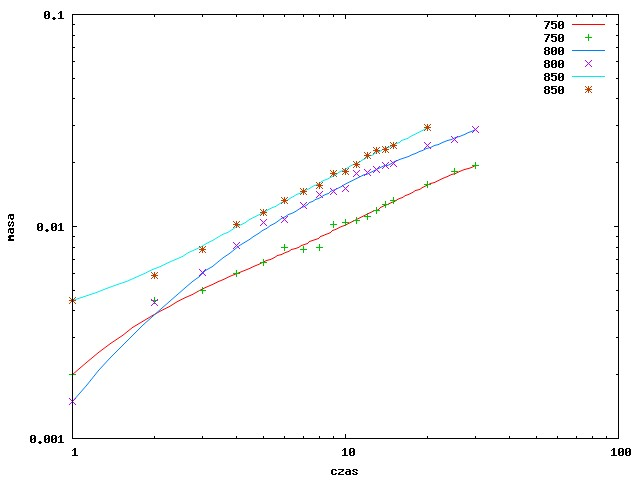
\includegraphics[scale=0.7]{all.jpg}
\label{rys1}
\end{figure}
\end{center}
Wszystkie badane próbki miały takie same wymiary i wynosiły one:\\
\begin{itemize}
\item szerokość: 0.8cm
\item długość: 4.8cm
\item grubość: 1mm
\end{itemize}
\section{Opracowanie wyników}
Następnie obliczamy nachylenia prawie-prostych korzystając z równania:\\
$$\log(\dfrac{\Delta m}{A})=\dfrac{1}{n}\log(t)$$
Wyniki przedstawia poniższa tabela:\\
\begin{tabular}{|c|c|c|c|}
\hline
$T$&$n_{750}$&$n_{800}$&$n_{850}$\\
\hline
2&-0.0848798461566&-0.0864510842858&-0.0792527355854\\
3&-0.112382482883&-0.128464436981&-0.130157260794\\
4&-0.152633448127&-0.165244356051&-0.168915303752\\
5&-0.172952756336&-0.195092892566&-0.185482325935\\
6&-0.20131709396&-0.179197491258&-0.208041656647\\
7&blad pomiarowy&-0.227541830991&-0.222490557332\\
8&-0.194486742928&-0.241444496687&-0.226324719858\\
9&-0.264915773679&-0.229036630272&-0.264915773679\\
10&-0.22384577977&-0.230286195864&-0.230286195864\\
11&-0.224271195964&-0.295053104981&-0.274169419348\\
12&-0.254193387345&-0.241570167535&-0.297930087794\\
13&-0.271734285086&-0.262381351669&-0.28540037663\\
14&-0.283597295528&-0.287232845378&-0.246826685988\\
15&-0.277019844499&-0.270837582037&-0.304268963635\\
20&-0.366844591794&-0.391730976454&-0.400870410572\\
25&-0.392209189439&-0.376393997061&blad pomiarowy\\
30&-0.382149046577&-0.426007293988&blad pomiarowy\\
\hline
\end{tabular}\\
Zauważamy, że $n$ nie jest stałe i ulega zmianie podczas prowadzenia eksperymentu.
\section{Wnioski}
Doświadczenie pokazało nam, że w podwyższonej temperaturze występuje przyśpieszona korozja metali.\\
Zauważyliśmy również, że tempo korozji jest zależne od temperatury.\\
Jednak nie udało mi się wykazać, ażeby współczynnik potęgowy n był równy 2, co uniemożliwia założenie że korozja miała charakter paraboliczny.
\end{document}
